% Section 3 -- the method.  Draft 5 Oct 2026; 13 Oct: numerical checks and implementation details moved to Appendix A (app:impl).  Every statement here is checked numerically in mathcheck/ (file named
% at the end of each property).  Terminology (review of 5 Oct): the exact route-V transfer is the REFERENCE
% construction; the network uses an inexpensive approximation of it ("route-V-inspired"), never "a gamblet construction".
\section{An operator-adapted learned V-cycle}\label{sec:method}

\subsection{Setting}\label{sec:setting}
We consider the family of elliptic problems
\begin{equation}\label{eq:pde}
  -\nabla\cdot\big(K(x)\nabla u\big) = f \quad\text{in } \Omega, \qquad u = 0 \text{ on } \Gamma_D,
  \qquad K\nabla u\cdot n = 0 \text{ on } \Gamma_N,
\end{equation}
with a symmetric, uniformly positive definite coefficient $K$ that is piecewise constant on the elements and may vary
by several orders of magnitude (isotropic $K = a\,I$ with high-contrast channels or barriers, or tensor-valued, strongly
anisotropic tows); a preliminary plane-strain elasticity case is treated in the same way (\appref{app:settings}). Starting from an
unstructured coarse triangulation $\mathcal{T}_0$ of $\Omega$, $L$ uniform refinements give nested $P_1$ spaces
$V_0\subset V_1\subset\cdots\subset V_L$. On level $k$ the nodes of $V_{k-1}$ (``coarse'', $C$) are ordered before the
nodes created by the refinement (``fine'', $F$), and the geometric prolongation is
$P_k = \begin{bmatrix} I \\ P_{k,F}\end{bmatrix}$, $P_{k,F}$ being nodal interpolation at edge midpoints.

On the finest level the discrete problem is $A u = F$, $A = A_L$ symmetric positive definite. A Galerkin solve on the
level-$k_0$ space gives $u_c$; we write $r = F - A u_c$ and $e = u - u_c = A^{-1} r$. The learned map studied here
returns a correction $c = \mathcal{N}(r; A)\approx e$ in one pass. The case $k_0 = 0$ means that \emph{no external coarse
solution is supplied} ($u_c = 0$, $r = F$); the network still contains its own exact coarsest-level solve.

Table~\ref{tab:notation} collects the notation.
\begin{table}[tbp]\centering\footnotesize
\caption{Notation.}\label{tab:notation}
\begin{tabular}{@{}>{\raggedright\arraybackslash}p{0.27\linewidth}>{\raggedright\arraybackslash}p{0.68\linewidth}@{}}\toprule
$A = A_L$, $A_k$ & fine operator; Galerkin operator on level $k$ ($A_0$ coarsest, solved exactly) \\
$D_k$, $W_{ij}$ & diagonal of $A_k$; normalised couplings $A_{ij}/A_{ii}$ (smoother inputs) \\
$P_k$, $\widehat\Phi_k$, $\Phi_k^\star$ & geometric, computational (eq.~\eqref{eq:jacobi}) and ideal (eq.~\eqref{eq:ideal}) prolongation \\
$u$, $u_c$, $r$, $e$ & discrete solution, level-$k_0$ Galerkin approximation, $r = F - Au_c$, $e = u - u_c$ \\
$Z$, $x_0$ & near-kernel indicator vectors; deflation \eqref{eq:deflation} \\
$x, x_c, x_p$ & pre-smoothing, coarse-correction and post-smoothing parts of the finest-level cycle \\
$\mathcal{S}^{\mathrm{pre}}, \mathcal{S}^{\mathrm{post}}$ & learned smoothers \eqref{eq:smoother} \\
$\|v\|_A$, $e(\hat u)$ & energy norm $\sqrt{v^\top Av}$; relative energy error $\|u - \hat u\|_A/\|u\|_A$ \\
$G$, $W$ (Section~\ref{sec:protocol}) & paired geometric-mean error ratio; win fraction \\
\bottomrule\end{tabular}
\end{table}

\subsection{Reference construction: ideal (route-V) transfers}\label{sec:routev}
Write the level-$k$ operator in the $C/F$ ordering as
$A_k = \begin{bmatrix} A_{CC} & A_{CF}\\ A_{FC} & A_{FF}\end{bmatrix}$ and define
\begin{multline}\label{eq:ideal}
  \Phi_k^\star = \begin{bmatrix} I\\ -A_{FF}^{-1}A_{FC}\end{bmatrix}, \qquad
  E_F = \begin{bmatrix} 0\\ I\end{bmatrix}, \qquad S_k = (\Phi_k^\star)^{\!\top} A_k \Phi_k^\star\\
  = A_{CC}-A_{CF}A_{FF}^{-1}A_{FC}.
\end{multline}
\begin{lemma}[two-level block diagonalisation]\label{lem:routev}
$E_F^\top A_k \Phi_k^\star = 0$, hence
\[
[\Phi_k^\star\;E_F]^\top A_k [\Phi_k^\star\;E_F] = \operatorname{diag}(S_k, A_{FF})
\]
and
\begin{equation}\label{eq:inverse}
  A_k^{-1} = \Phi_k^\star S_k^{-1} (\Phi_k^\star)^{\!\top} + E_F A_{FF}^{-1} E_F^\top .
\end{equation}
\end{lemma}
\begin{proof}
$E_F^\top A_k\Phi_k^\star = A_{FC} - A_{FF}A_{FF}^{-1}A_{FC} = 0$. The matrix $T = [\Phi_k^\star\;E_F]$ is unit block
lower triangular, hence invertible, and $T^\top A_k T$ is block diagonal; inverting
$A_k = T^{-\top}\operatorname{diag}(S_k,A_{FF})T^{-1}$ gives \eqref{eq:inverse}.
\end{proof}
Applied recursively with $A_{k-1} = S_k$, \eqref{eq:inverse} is the exact multilevel decomposition behind
operator-adapted wavelets \cite{amaratunga2006,sudarshan2005thesis,dheedene2005thesis} and, with nodal measurement functions, gamblets
\cite{owhadi2017}: the columns of $\Phi_k^\star$ are $A$-harmonic extensions of the coarse nodal values. It is also the
ideal interpolation of algebraic multigrid. Two remarks fix how it is used here. First, \eqref{eq:inverse} restricts with $\Phi^\top$ and prolongs with $\Phi$, so we
pass residuals down with $\widehat\Phi_k^{\!\top}$ (the contrast with exactly invertible lifting networks is discussed in
\appref{app:impl}). Second, $\Phi_k^\star$ is dense in general and its decay with distance depends on the contrast
unless the coarse space resolves the high-conductivity structures \cite{hellman2017,peterseim2016}. We therefore use
\eqref{eq:ideal} as the reference and compute an inexpensive approximation.

\paragraph{Computational transfer.} Starting from the geometric predict, $m$ weighted-Jacobi steps are applied to
$A_{FF}X = -A_{FC}$:
\begin{equation}\label{eq:jacobi}
  X^{(0)} = P_{k,F}, \quad X^{(j+1)} = X^{(j)} + \omega D_{FF}^{-1}\big(-A_{FC} - A_{FF}X^{(j)}\big), \quad
  \widehat\Phi_k = \begin{bmatrix} I\\ X^{(m)}\end{bmatrix},
\end{equation}
with $D_{FF} = \operatorname{diag}(A_{FF})$, $\omega = 2/3$, $m = 4$ (prolongator smoothing in the sense of smoothed
aggregation \cite{vanek1996}). The number of steps $m$ controls the stencil width of $\widehat\Phi_k$ and how closely it
approximates $\Phi_k^\star$; increasing $m$ approaches the ideal prolongation only when the Jacobi iteration for $A_{FF}$
converges, which symmetric positive definiteness alone does not guarantee for a fixed weight. $m = 4$ was fixed during
development, and its measured effect on the classical reference, the learned margin, the operator complexity and the set-up
time is reported in \appref{app:sensitivity}. The coarse operators are Galerkin, $A_{k-1} = \widehat\Phi_k^{\!\top} A_k\widehat\Phi_k$,
and the hierarchy is computed per sample from $A$ alone.
\begin{proposition}[local reproduction of the kernel]\label{prop:constants}
Let $t$ be a level-$k$ vector with restriction $t_C$ to the coarse nodes (constants for diffusion; translations and
rotations for elasticity, which $P_1$ interpolation reproduces), and let $\mathcal{N}_r(f)$ denote the nodes within $r$
graph steps of a fine node $f$. If $P_k t_C = t$ on $\mathcal{N}_m(f)$ and $(A_k t)_g = 0$ for every fine node
$g\in\mathcal{N}_{m-1}(f)$, then $(\widehat\Phi_k t_C)_f = t_f$.
\end{proposition}
\begin{proof}
Write $\widehat\Phi^{(j)} = [I;X^{(j)}]$; the update in \eqref{eq:jacobi} applied to $t_C$ at a fine node $g$ is
$-\omega\,(A_k\widehat\Phi^{(j)}t_C)_g/A_{gg}$, which depends on $\widehat\Phi^{(j)}t_C$ on $\mathcal{N}_1(g)$ only. We
show by induction that $\widehat\Phi^{(j)}t_C = t$ on $\mathcal{N}_{m-j}(f)$. For $j = 0$ this is the hypothesis. If it
holds for $j$ and $g\in\mathcal{N}_{m-j-1}(f)$, then $\mathcal{N}_1(g)\subset\mathcal{N}_{m-j}(f)$, so the update at $g$ is
$-\omega(A_kt)_g/A_{gg} = 0$ and $\widehat\Phi^{(j+1)}t_C = t$ on $\mathcal{N}_{m-j-1}(f)$. Take $j = m$.
\end{proof}
The statement is graph-local and conditional; the measured reproduction defects of the elasticity transfers, at round-off
on most finest-level rows and growing on coarser levels, are reported in \appref{app:impl}.

\subsection{The learned cycle}\label{sec:cycle}
For $k = L, L-1, \dots, 1$ and a right-hand side $b$ on level $k$, one cycle returns three parts,
\begin{equation}\label{eq:cycle}
\begin{aligned}
  x &= \mathcal{S}^{\mathrm{pre}}(b; A_k), &
  e_c &= \mathcal{C}_{k-1}\big(\widehat\Phi_k^{\!\top}(b - A_k x)\big), &
  x_c &= \widehat\Phi_k e_c, \\
  x_p &= \mathcal{S}^{\mathrm{post}}\big(b - A_k(x + x_c); A_k\big), &
  \mathcal{C}_k(b) &= x + x_c + x_p, & \mathcal{C}_0 &= A_0^{-1},
\end{aligned}
\end{equation}
with an exact dense solve on the coarsest level (28 nodes for the perforated square, 45 for the polygon). Only the smoothers are learned. The transfers are computed deterministically from each sample with the approximate
construction \eqref{eq:jacobi}; the Galerkin operators, residual updates and the coarsest solve are fixed algebraic
operations on them.

\paragraph{Smoother.} A smoother maps a right-hand side $b$ on a level with operator $A_k$ to a correction. With
$d = \operatorname{diag}(A_k)$, $z = b/d$ and $\sigma = \|z\|_{\mathrm{rms}}$, node features are
$(z_i/\sigma,\ \log(d_i/\operatorname{median} d))$; an encoder lifts them to a latent $s\in\mathbb{R}^{n\times C}$, and
$T$ steps of
\begin{equation}\label{eq:smoother}
\begin{aligned}
  s_i \leftarrow s_i &+ \mathcal{L}_t\big([\,s_i,\ \textstyle\sum_{j\ne i} W_{ij} V_t s_j\,]\big)\\
       &+ \mathcal{M}_t\big([\,s_i,\ \textstyle\sum_{j\ne i} W_{ij} V_t s_j,\ \overline{m}_i\,]\big),
  \qquad W_{ij} = A_{ij}/A_{ii},
\end{aligned}
\end{equation}
follow, where $\mathcal{L}_t$ and $V_t$ are linear, $\mathcal{M}_t$ is a small MLP and $\overline{m}_i$ the mean of edge
messages $\mathrm{MLP}([s_i,s_j,\delta_{ij},|\delta_{ij}|,W_{ij}])$ over the neighbours of $i$, with
$\delta_{ij} = (\mathbf{x}_j-\mathbf{x}_i)/h_k$ the edge vector in units of the level's mesh width. The output is $\sigma\cdot\mathrm{dec}(s)$. The operator
enters only through $W$ and $d$ of the level the smoother acts on; one pre- and one post-smoother are shared by all
levels ($T = \nu = 4$, $C$ chosen to meet the parameter budget).

\subsection{Near-kernel deflation from the operator}\label{sec:deflation}
High-contrast media can contain \emph{floating islands}: conductive regions enclosed by low-conductivity barriers and
not connected to $\Gamma_D$. Their indicator vectors $z$ satisfy $z^\top A z/z^\top D z \ll 1$, i.e.\ they lie close to the
kernel of $A$, and the nodal hierarchy used here does not contain them unless its coarse levels resolve the island. We detect
them from $A$ alone. Let $G$ be the graph of strong connections, $-A_{ij}\ge\theta\sqrt{A_{ii}A_{jj}}$ ($\theta = 0.1$). A
connected component of $G$ is \emph{anchored} if one of its rows is strongly coupled to the Dirichlet boundary,
$\sum_j A_{ij}\ge\theta A_{ii}$ (interior rows of a diffusion matrix sum to zero). The indicator of every unanchored
component with Rayleigh quotient $z^\top Az/z^\top Dz<\tau$ ($\tau = 0.05$) is a column of $Z$. Before the cycle,
\begin{equation}\label{eq:deflation}
  x_0 = Z(Z^\top A Z)^{-1}Z^\top r .
\end{equation}
If no vector is detected, $Z$ is empty and $x_0 = 0$ (no deflation); for the elasticity case $Z$ is always empty. The
indicators of distinct components have disjoint supports and positive energy, so $Z^\top AZ$ is nonsingular whenever $Z$ is
not empty.
Against the geometric ground truth (conductive elements, connected components without a Dirichlet node) the detector
has recall 74/75 and precision 75/78 on the barrier test set of the development data seed; the three additional vectors are near-kernel modes by
definition (Rayleigh quotients 0.008--0.015) but not coefficient islands (\texttt{mathcheck/check\_oa\_vcp.log}).
The detector is a heuristic for scalar diffusion matrices: the strength criterion uses negative off-diagonal couplings
and the anchoring test the zero row sums of interior rows. A small Rayleigh quotient certifies that a returned vector has
low energy; it does not certify that every important low-energy direction was found. For tensor coefficients (whose
$P_1$ matrices need not be M-matrices) we report how many vectors it returns, and for elasticity it is not used. The
thresholds were fixed on the development seed and are kept in all main experiments; a subsequent sensitivity check on the
held-out barrier sets (\appref{app:sensitivity}) shows that $\theta$ matters more than $\tau$ and that the learned margin
changes little ($G = 2.03$ against $2.00$ with $\theta = 0.05$).

\subsection{Galerkin output and training}\label{sec:output}
The cycle is applied to the deflated residual $b = r - Ax_0$ on the finest level, and its parts are combined
energy-optimally together with the near-kernel vectors:
\begin{equation}\label{eq:projection}
  W = [\,x,\ x_c,\ x_p,\ Z\,], \qquad c = x_0 + W y, \qquad W^\top A W\, y = W^\top (r - A x_0).
\end{equation}
If the columns of $W$ are linearly dependent (a vanishing part, say), the normal equations remain consistent and
determine $Wy$, the $A$-orthogonal projection onto $\operatorname{span}W$, uniquely, although $y$ need not be unique; as a
mathematical convention we take $y = (W^\top AW)^{+}W^\top(r - Ax_0)$, and any rank-revealing solve gives the same $c$. The small
Gram system and its right-hand side are formed and solved in double precision, after Jacobi scaling of its columns; the
regularisation and acceptance step of the implementation are described in \appref{app:impl}. Training minimises
$\ell(c) + \ell(x_0 + x + x_c + x_p)$ with $\ell$ the mean of the relative $L^2$ and energy errors. The second term keeps
each part of the cycle well scaled; training through the projection alone makes the loss insensitive to the scale of the
parts and stalls on the channel problems (variant \texttt{oa-vcp}, development-stage CPU screen on a two-level mesh, \path{diagnostics_cost/oa_vcp_L2_cpu.log}).

\paragraph{Summary of one pass.} Algorithm~\ref{alg:opdata} lists the operator data computed for each sample and
Algorithm~\ref{alg:pass} one pass of the network; Figure~\ref{fig:schematic} shows how they fit together. Everything except
the two smoothers is a prescribed algebraic operation: the transfers, Galerkin levels, coarsest factorisation and deflation
vectors are computed from the operator of the sample before the pass, while the deflation step, residual updates and output
projection act on the residual and on the parts produced by the smoothers. Both algorithms and the figure show the ideal
mathematical construction, with exact solves of the small deflation and normal-equation systems; the regularisation and
acceptance step of the implementation are described in \appref{app:impl}.
\begin{algorithm}[tbp]
\caption{Operator data for one sample (computed from $A = A_L$; no learned parameters).}\label{alg:opdata}
\begin{algorithmic}[1]
\Require fine operator $A_L$; geometric prolongations $P_k = [I;\,P_{k,F}]$; number of levels; $m = 4$, $\omega = 2/3$
\For{$k = L, L-1, \dots, 1$}
  \State split $A_k$ into $C/F$ blocks; $X \gets P_{k,F}$
  \For{$j = 1,\dots,m$} \State $X \gets X + \omega D_{FF}^{-1}(-A_{FC} - A_{FF}X)$ \Comment{eq.~\eqref{eq:jacobi}} \EndFor
  \State $\widehat\Phi_k \gets [I;\,X]$, \quad $A_{k-1} \gets \widehat\Phi_k^{\!\top}A_k\widehat\Phi_k$ \Comment{Galerkin level}
  \State $d_k \gets \operatorname{diag}(A_k)$, \quad $W^{(k)}_{ij} \gets A_{ij}/A_{ii}$ \Comment{smoother inputs}
\EndFor
\State factor $A_0$ (dense, exact)
\State $Z \gets$ indicators of the unanchored strong-connection components of $A_L$ with Rayleigh quotient $<\tau$ \Comment{Section~\ref{sec:deflation}}
\end{algorithmic}
\end{algorithm}
\begin{algorithm}[tbp]
\caption{One OA-VCB pass, ideal construction (exact small solves; for the regularised implementation see
\appref{app:impl}). $\mathcal{S}^{\mathrm{pre}},\mathcal{S}^{\mathrm{post}}$ are the learned smoothers
\eqref{eq:smoother}, shared by all levels. If $Z$ is empty, $x_0 = 0$; if $W$ is rank-deficient, $y$ is the
pseudoinverse solution, and $Wy$ is unique.}\label{alg:pass}
\begin{algorithmic}[1]
\Require residual $r = F - Au_c$; operator data of Algorithm~\ref{alg:opdata}
\State $x_0 \gets Z(Z^{\!\top}AZ)^{-1}Z^{\!\top}r$, \quad $b \gets r - Ax_0$ \Comment{deflation \eqref{eq:deflation}}
\State $(x, x_c, x_p) \gets \textsc{Cycle}(L, b)$ \Comment{parts on the finest level}
\State $W \gets [\,x,\ x_c,\ x_p,\ Z\,]$; solve $W^{\!\top}AW\,y = W^{\!\top}b$ \Comment{Galerkin output \eqref{eq:projection}}
\State \Return $\hat u = u_c + x_0 + Wy$
\Function{Cycle}{$k$, $b$}
  \If{$k = 0$} \Return $A_0^{-1}b$ \EndIf
  \State $x \gets \mathcal{S}^{\mathrm{pre}}(b; A_k)$
  \State $x_c \gets \widehat\Phi_k\,\textsc{Cycle}\big(k-1,\ \widehat\Phi_k^{\!\top}(b - A_kx)\big)$
  \State $x_p \gets \mathcal{S}^{\mathrm{post}}\big(b - A_k(x + x_c); A_k\big)$
  \State \Return $(x, x_c, x_p)$ if $k = L$, else $x + x_c + x_p$
\EndFunction
\end{algorithmic}
\end{algorithm}
\begin{figure}[tbp]\centering
\resizebox{\linewidth}{!}{% Schematic of OA-VCB (TikZ), 11 Oct 2026.  Input with % Schematic of OA-VCB (TikZ), 11 Oct 2026.  Input with % Schematic of OA-VCB (TikZ), 11 Oct 2026.  Input with \input{figures/fig_schematic} inside a figure environment.
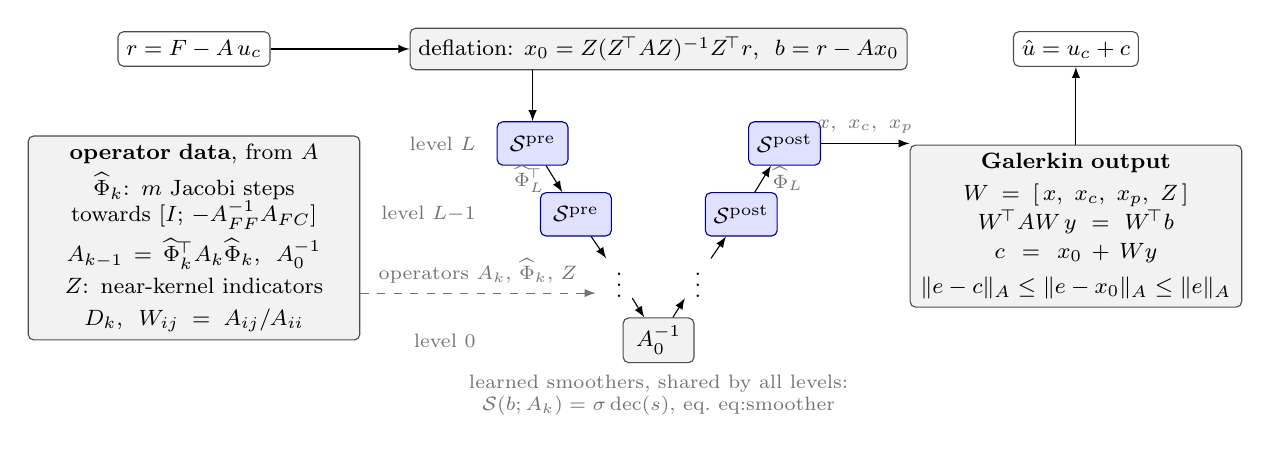
\begin{tikzpicture}[x=1cm, y=1cm, font=\footnotesize, >=latex,
  box/.style={draw=black!70, rounded corners=2pt, align=center, inner sep=3pt},
  op/.style={box, fill=black!5},
  learn/.style={box, fill=blue!12, draw=blue!60!black, minimum width=9mm, minimum height=5.5mm},
  lvl/.style={font=\scriptsize, text=black!55}]
% left: operator data
\node[box] (in) at (1.80,2.55) {$r = F - A\,u_c$};
\node[op, text width=40mm] (data) at (1.80,0.15) {\textbf{operator data}, from $A$\\[2pt]
  $\widehat\Phi_k$: $m$ Jacobi steps\\ towards $[I;\,-A_{FF}^{-1}A_{FC}]$\\[2pt]
  $A_{k-1}=\widehat\Phi_k^{\!\top}A_k\widehat\Phi_k$, \ $A_0^{-1}$\\[2pt]
  $Z$: near-kernel indicators\\[2pt] $D_k$, \ $W_{ij}=A_{ij}/A_{ii}$};
% middle: deflation and V-cycle
\node[op] (defl) at (7.70,2.55) {deflation: $x_0 = Z(Z^{\!\top}AZ)^{-1}Z^{\!\top}r$, \ $b = r - Ax_0$};
\node[learn] (s3) at (6.10,1.35) {$\mathcal{S}^{\mathrm{pre}}$};   \node[learn] (p3) at (9.30,1.35) {$\mathcal{S}^{\mathrm{post}}$};
\node[learn] (s2) at (6.65,0.45) {$\mathcal{S}^{\mathrm{pre}}$};  \node[learn] (p2) at (8.75,0.45) {$\mathcal{S}^{\mathrm{post}}$};
\node (s1) at (7.20,-0.35) {$\vdots$};                            \node (p1) at (8.20,-0.35) {$\vdots$};
\node[op, minimum width=9mm] (c0) at (7.70,-1.15) {$A_0^{-1}$};
\draw[->] (s3) -- node[left, lvl] {$\widehat\Phi_L^{\!\top}$} (s2);  \draw[->] (s2) -- (s1);  \draw[->] (s1) -- (c0);
\draw[->] (c0) -- (p1); \draw[->] (p1) -- (p2); \draw[->] (p2) -- node[right, lvl] {$\widehat\Phi_L$} (p3);
\node[lvl, anchor=east] at (5.50,1.35) {level $L$}; \node[lvl, anchor=east] at (5.50,0.45) {level $L{-}1$};
\node[lvl, anchor=east] at (5.50,-1.15) {level $0$};
\draw[->] (defl.south -| s3) -- (s3);
\node[lvl, align=center] at (7.70,-1.85) {learned smoothers, shared by all levels:\\ $\mathcal{S}(b;A_k) = \sigma\,\mathrm{dec}(s)$, eq.~\eqref{eq:smoother}};
% right: Galerkin output
\node[op, text width=40mm] (out) at (13.00,0.30) {\textbf{Galerkin output}\\[2pt]
  $W=[\,x,\ x_c,\ x_p,\ Z\,]$\\[1pt] $W^{\!\top}AW\,y = W^{\!\top}b$\\[1pt] $c = x_0 + Wy$\\[3pt]
  $\|e-c\|_A\le\|e-x_0\|_A\le\|e\|_A$};
\node[box] (res) at (13.00,2.55) {$\hat u = u_c + c$};
% connections
\draw[->] (in) -- (defl);
\draw[->, dashed, black!55] (data.east |- 0,-0.55) -- node[above, lvl] {operators $A_k$, $\widehat\Phi_k$, $Z$} (6.9,-0.55);
\draw[->] (p3.east) -- node[above, lvl] {$x,\ x_c,\ x_p$} (out.west |- p3.east);
\draw[->] (out) -- (res);
\end{tikzpicture}
 inside a figure environment.
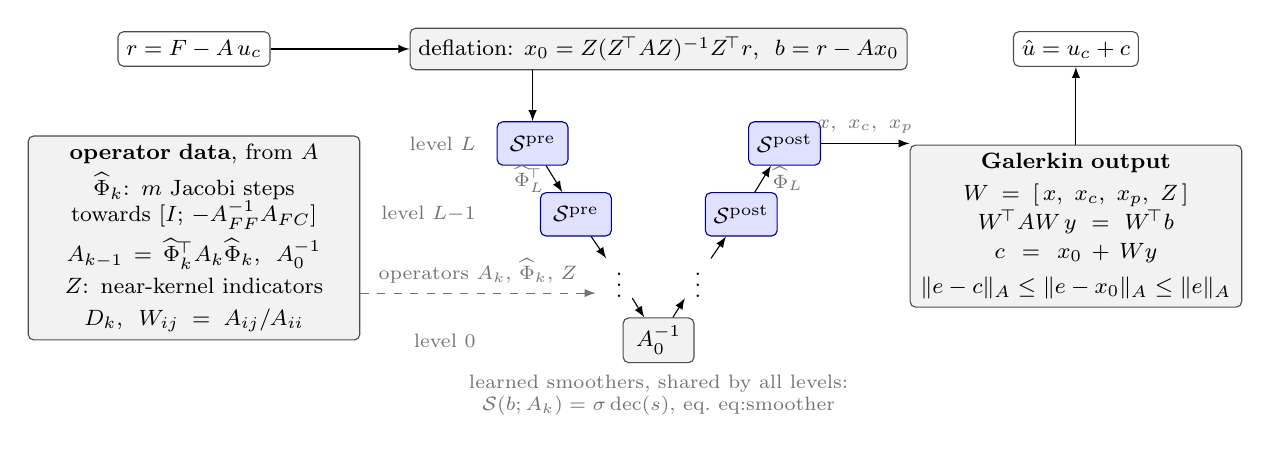
\begin{tikzpicture}[x=1cm, y=1cm, font=\footnotesize, >=latex,
  box/.style={draw=black!70, rounded corners=2pt, align=center, inner sep=3pt},
  op/.style={box, fill=black!5},
  learn/.style={box, fill=blue!12, draw=blue!60!black, minimum width=9mm, minimum height=5.5mm},
  lvl/.style={font=\scriptsize, text=black!55}]
% left: operator data
\node[box] (in) at (1.80,2.55) {$r = F - A\,u_c$};
\node[op, text width=40mm] (data) at (1.80,0.15) {\textbf{operator data}, from $A$\\[2pt]
  $\widehat\Phi_k$: $m$ Jacobi steps\\ towards $[I;\,-A_{FF}^{-1}A_{FC}]$\\[2pt]
  $A_{k-1}=\widehat\Phi_k^{\!\top}A_k\widehat\Phi_k$, \ $A_0^{-1}$\\[2pt]
  $Z$: near-kernel indicators\\[2pt] $D_k$, \ $W_{ij}=A_{ij}/A_{ii}$};
% middle: deflation and V-cycle
\node[op] (defl) at (7.70,2.55) {deflation: $x_0 = Z(Z^{\!\top}AZ)^{-1}Z^{\!\top}r$, \ $b = r - Ax_0$};
\node[learn] (s3) at (6.10,1.35) {$\mathcal{S}^{\mathrm{pre}}$};   \node[learn] (p3) at (9.30,1.35) {$\mathcal{S}^{\mathrm{post}}$};
\node[learn] (s2) at (6.65,0.45) {$\mathcal{S}^{\mathrm{pre}}$};  \node[learn] (p2) at (8.75,0.45) {$\mathcal{S}^{\mathrm{post}}$};
\node (s1) at (7.20,-0.35) {$\vdots$};                            \node (p1) at (8.20,-0.35) {$\vdots$};
\node[op, minimum width=9mm] (c0) at (7.70,-1.15) {$A_0^{-1}$};
\draw[->] (s3) -- node[left, lvl] {$\widehat\Phi_L^{\!\top}$} (s2);  \draw[->] (s2) -- (s1);  \draw[->] (s1) -- (c0);
\draw[->] (c0) -- (p1); \draw[->] (p1) -- (p2); \draw[->] (p2) -- node[right, lvl] {$\widehat\Phi_L$} (p3);
\node[lvl, anchor=east] at (5.50,1.35) {level $L$}; \node[lvl, anchor=east] at (5.50,0.45) {level $L{-}1$};
\node[lvl, anchor=east] at (5.50,-1.15) {level $0$};
\draw[->] (defl.south -| s3) -- (s3);
\node[lvl, align=center] at (7.70,-1.85) {learned smoothers, shared by all levels:\\ $\mathcal{S}(b;A_k) = \sigma\,\mathrm{dec}(s)$, eq.~\eqref{eq:smoother}};
% right: Galerkin output
\node[op, text width=40mm] (out) at (13.00,0.30) {\textbf{Galerkin output}\\[2pt]
  $W=[\,x,\ x_c,\ x_p,\ Z\,]$\\[1pt] $W^{\!\top}AW\,y = W^{\!\top}b$\\[1pt] $c = x_0 + Wy$\\[3pt]
  $\|e-c\|_A\le\|e-x_0\|_A\le\|e\|_A$};
\node[box] (res) at (13.00,2.55) {$\hat u = u_c + c$};
% connections
\draw[->] (in) -- (defl);
\draw[->, dashed, black!55] (data.east |- 0,-0.55) -- node[above, lvl] {operators $A_k$, $\widehat\Phi_k$, $Z$} (6.9,-0.55);
\draw[->] (p3.east) -- node[above, lvl] {$x,\ x_c,\ x_p$} (out.west |- p3.east);
\draw[->] (out) -- (res);
\end{tikzpicture}
 inside a figure environment.
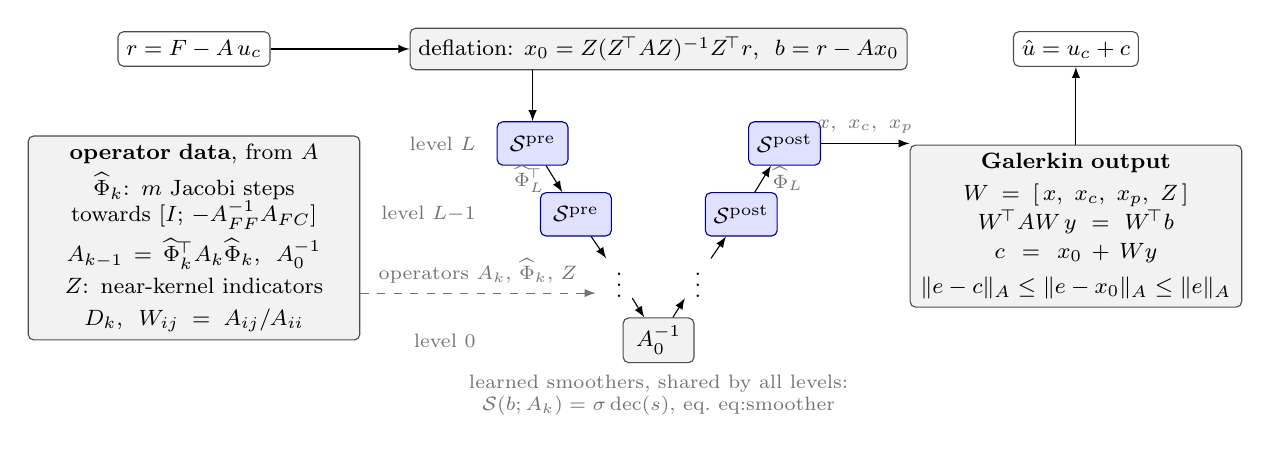
\begin{tikzpicture}[x=1cm, y=1cm, font=\footnotesize, >=latex,
  box/.style={draw=black!70, rounded corners=2pt, align=center, inner sep=3pt},
  op/.style={box, fill=black!5},
  learn/.style={box, fill=blue!12, draw=blue!60!black, minimum width=9mm, minimum height=5.5mm},
  lvl/.style={font=\scriptsize, text=black!55}]
% left: operator data
\node[box] (in) at (1.80,2.55) {$r = F - A\,u_c$};
\node[op, text width=40mm] (data) at (1.80,0.15) {\textbf{operator data}, from $A$\\[2pt]
  $\widehat\Phi_k$: $m$ Jacobi steps\\ towards $[I;\,-A_{FF}^{-1}A_{FC}]$\\[2pt]
  $A_{k-1}=\widehat\Phi_k^{\!\top}A_k\widehat\Phi_k$, \ $A_0^{-1}$\\[2pt]
  $Z$: near-kernel indicators\\[2pt] $D_k$, \ $W_{ij}=A_{ij}/A_{ii}$};
% middle: deflation and V-cycle
\node[op] (defl) at (7.70,2.55) {deflation: $x_0 = Z(Z^{\!\top}AZ)^{-1}Z^{\!\top}r$, \ $b = r - Ax_0$};
\node[learn] (s3) at (6.10,1.35) {$\mathcal{S}^{\mathrm{pre}}$};   \node[learn] (p3) at (9.30,1.35) {$\mathcal{S}^{\mathrm{post}}$};
\node[learn] (s2) at (6.65,0.45) {$\mathcal{S}^{\mathrm{pre}}$};  \node[learn] (p2) at (8.75,0.45) {$\mathcal{S}^{\mathrm{post}}$};
\node (s1) at (7.20,-0.35) {$\vdots$};                            \node (p1) at (8.20,-0.35) {$\vdots$};
\node[op, minimum width=9mm] (c0) at (7.70,-1.15) {$A_0^{-1}$};
\draw[->] (s3) -- node[left, lvl] {$\widehat\Phi_L^{\!\top}$} (s2);  \draw[->] (s2) -- (s1);  \draw[->] (s1) -- (c0);
\draw[->] (c0) -- (p1); \draw[->] (p1) -- (p2); \draw[->] (p2) -- node[right, lvl] {$\widehat\Phi_L$} (p3);
\node[lvl, anchor=east] at (5.50,1.35) {level $L$}; \node[lvl, anchor=east] at (5.50,0.45) {level $L{-}1$};
\node[lvl, anchor=east] at (5.50,-1.15) {level $0$};
\draw[->] (defl.south -| s3) -- (s3);
\node[lvl, align=center] at (7.70,-1.85) {learned smoothers, shared by all levels:\\ $\mathcal{S}(b;A_k) = \sigma\,\mathrm{dec}(s)$, eq.~\eqref{eq:smoother}};
% right: Galerkin output
\node[op, text width=40mm] (out) at (13.00,0.30) {\textbf{Galerkin output}\\[2pt]
  $W=[\,x,\ x_c,\ x_p,\ Z\,]$\\[1pt] $W^{\!\top}AW\,y = W^{\!\top}b$\\[1pt] $c = x_0 + Wy$\\[3pt]
  $\|e-c\|_A\le\|e-x_0\|_A\le\|e\|_A$};
\node[box] (res) at (13.00,2.55) {$\hat u = u_c + c$};
% connections
\draw[->] (in) -- (defl);
\draw[->, dashed, black!55] (data.east |- 0,-0.55) -- node[above, lvl] {operators $A_k$, $\widehat\Phi_k$, $Z$} (6.9,-0.55);
\draw[->] (p3.east) -- node[above, lvl] {$x,\ x_c,\ x_p$} (out.west |- p3.east);
\draw[->] (out) -- (res);
\end{tikzpicture}
}
\caption{One OA-VCB pass, ideal construction. Grey boxes denote prescribed algebraic operations; blue boxes denote the learned
smoothers, one pre- and one post-smoother shared by all levels. The operator-data box is precomputed from each sample's
operator (Algorithm~\ref{alg:opdata}); deflation and the Galerkin output depend on the residual and on the cycle's parts. The
output is the energy-optimal combination of the three parts and the near-kernel vectors, which gives the safeguard of
Proposition~\ref{prop:safeguard}; the regularisation and acceptance step of the implementation are described in
\appref{app:impl}.}
\label{fig:schematic}
\end{figure}

\subsection{Properties}\label{sec:properties}
\begin{proposition}[containment of fixed polynomial smoothers]\label{prop:containment}
Let $\nu\ge1$ steps and $C\ge2$ latent channels be given, and let $p(\mu) = \sum_{j=0}^{\nu-1}a_j\mu^j$ be any real
polynomial of degree at most $\nu-1$. Set the encoder, the step maps and the decoder of both smoothers as follows: channel $1$
of the latent carries $z/\sigma$, channel $0$ starts at zero, $V_t$ selects channel $0$, $\mathcal{L}_t$ maps $(s,\,q)$ to
$a_{\nu-t}\,s_1 + q_0$ in channel $0$ and to zero elsewhere, $\mathcal{M}_t = 0$, and the decoder reads channel $0$. Then on
every level each smoother returns
\begin{equation}\label{eq:polysmoother}
\begin{aligned}
  x &= p(B_k)\,D_k^{-1}b, & B_k &= D_k^{-1}A_k,\\
  A_k^{-1}b - x &= R(B_k)\,A_k^{-1}b, & R(\mu) &= 1 - \mu\,p(\mu),
\end{aligned}
\end{equation}
with the same coefficients on all levels; and the network output \eqref{eq:deflation}--\eqref{eq:projection} equals the
classical deflated V$(\nu,\nu)$ cycle with these smoothers, transfers \eqref{eq:jacobi}, Galerkin levels, exact coarsest solve
and Galerkin projection onto $\operatorname{span}\{x,x_c,x_p,Z\}$. Equivalently, every real residual polynomial $R$ of degree at
most $\nu$ with $R(0) = 1$ is represented. When $R$ has real roots $1/\omega_t$, the step maps
$\mathcal{L}_t(s,q) = \omega_t(s_1 - s_0 - q_0)$ in channel $0$ realise the same smoother as the Richardson steps
\begin{equation}\label{eq:richardson}
  x \leftarrow x + \omega_t D_k^{-1}(b - A_k x), \qquad t = 1,\dots,\nu, \qquad x = 0 \text{ initially},
\end{equation}
for which $R(\mu) = \prod_{t=1}^{\nu}(1 - \omega_t\mu)$. Special cases are
\begin{enumerate}
\item[(a)] weighted Jacobi smoothing, $\omega_t = \omega$;
\item[(b)] degree-$\nu$ Chebyshev smoothing on a fixed interval $[\lambda/q,\lambda]$ with $\lambda>0$ and $q>1$,
$\omega_t^{-1} = \theta - \delta\cos\big((2t-1)\pi/(2\nu)\big)$, $\theta = (\lambda + \lambda/q)/2$, $\delta = (\lambda - \lambda/q)/2$,
for which $\prod_t(1-\omega_t\mu) = T_\nu\big((\theta-\mu)/\delta\big)/T_\nu(\theta/\delta)$, the residual polynomial of the
Chebyshev semi-iteration \cite{saad2003}.
\end{enumerate}
\end{proposition}
\begin{proof}
Write $s_0 = x/\sigma$ for channel $0$ at node $i$; its aggregate is $q_0 = \sum_{j\ne i}W_{ij}x_j/\sigma = \big((B_k - I)x\big)_i/\sigma$.
Since the step map is added to the current state, step $t$ of the first construction gives
$s_0 + a_{\nu-t}s_1 + q_0 = \big(B_kx + a_{\nu-t}D_k^{-1}b\big)_i/\sigma$, that is, $x_t = B_kx_{t-1} + a_{\nu-t}D_k^{-1}b$ with
$x_0 = 0$, and Horner's rule gives $x_\nu = \sum_{j=0}^{\nu-1}a_jB_k^{\,j}D_k^{-1}b = p(B_k)D_k^{-1}b$. Multiplying the decoded
channel by $\sigma$ undoes the scaling, and $A_k^{-1}b - p(B_k)B_kA_k^{-1}b = R(B_k)A_k^{-1}b$. Conversely, a real $R$ of degree
at most $\nu$ with $R(0) = 1$ has the form $1-\mu p(\mu)$ with $p$ real of degree at most $\nu-1$. In the second construction
step $t$ gives $s_0 + \omega_t(s_1 - s_0 - q_0) = \big(x + \omega_t D_k^{-1}(b - A_k x)\big)_i/\sigma$, and each step multiplies the
error $A_k^{-1}b - x$ by $I-\omega_tB_k$. The remaining operations in \eqref{eq:cycle}--\eqref{eq:projection} are the same in
the network and the classical cycle. For (b), both sides are polynomials of degree $\nu$ in $\mu$ that equal $1$ at $\mu = 0$
and vanish at the $\nu$ distinct Chebyshev nodes $\mu_t = \omega_t^{-1}$ of the interval, so they coincide.
\end{proof}
The construction requires the coefficients to be shared across levels, because the smoother parameters are; it does not
cover smoothers whose coefficients depend on the level or on the operator, and it bounds the degree by the number of steps.
Containment is a statement of representation: it does not assert that the represented cycle contracts, nor, in (b), that
$[\lambda/q,\lambda]$ encloses the spectrum of $B_k$ on every level. Equivalently, the containment bounds the correction polynomial $p$ by degree $\nu-1$ and the residual polynomial $R$ by
degree $\nu$ (three and four at $\nu = 4$); the learned nonlinear smoother itself has no polynomial degree, and the
proposition does not say that a smoother outside this class cannot be represented. Numerically the network with the weights
of the construction reproduces the classical cycles to about $10^{-10}$ (\appref{app:impl}). We call the cycles of (a) and (b) the \emph{contained Jacobi
member} and the \emph{contained fixed-interval Chebyshev member}.

\paragraph{Classical reference.} For the numerical comparisons we use the classical cycle that is customary in multigrid: the
same deflated V$(4,4)$ cycle with the same transfers, Galerkin levels, coarsest solve, coarse solution $u_c$ and Galerkin
output, with degree-4 Chebyshev smoothers whose spectral interval $[\lambda_k/10,\lambda_k]$ is set per level: $\lambda_k = 3$
on the finest scalar level and otherwise $1.05$ times a 30-step power-iteration estimate of the largest eigenvalue of
$D_k^{-1}A_k$, a heuristic spectral estimate rather than a certified upper bound. We call it the \emph{classical reference}.
Because its intervals depend on the level and the operator, Proposition~\ref{prop:containment} does not establish that it is
contained in the architecture. Numerically it is within a few per cent of the contained fixed-interval Chebyshev member
($\lambda = 3$ on all levels): on the test sets of Table~\ref{tab:contained}, the paired geometric-mean ratio of the
fixed-interval to the adaptive errors lies between $0.975$ and $1.056$, and the contained Jacobi member is $1.35$--$1.82$ times
less accurate (Table~\ref{tab:contained} in \appref{app:impl}). Comparing OA-VCB with this reference compares four learned
update stages per pre- and post-smoother with a degree-four Chebyshev smoother: a controlled architectural comparison, not one
at equal work and not an optimisation over all contained polynomials.
\begin{proposition}[positive homogeneity]\label{prop:homogeneity}
$\mathcal{N}(\lambda r; A) = \lambda\,\mathcal{N}(r; A)$ for every $\lambda > 0$.
\end{proposition}
\begin{proof}
For a smoother, $z$ and $\sigma$ scale with $\lambda$, the features $z/\sigma$ and $\log d$ do not, and the output carries
the factor $\sigma$; so $\mathcal{S}(\lambda b) = \lambda\mathcal{S}(b)$ (and $\mathcal{S}(0) = 0$ by definition). The residual updates, transfers, coarsest solve
and deflation \eqref{eq:deflation} are linear. In \eqref{eq:projection} every column of $W$ except $Z$ scales with
$\lambda$, so $\operatorname{span}W$ is unchanged and the projection of $\lambda(r - Ax_0)$ onto it is $\lambda$ times
the projection of $r - Ax_0$.
\end{proof}
Homogeneity concerns the scale of the data only; it says nothing about right-hand sides of a different shape
(Section~\ref{sec:rhs}), and it does not cover $\lambda<0$: the smoothers are not odd in $r$, so a reversed load
$-f$ is an off-load case like any other (the classical reference is odd in $r$, including after its Galerkin output projection). Numerically $|\mathcal{N}(2.5r)-2.5\mathcal{N}(r)|/|2.5\mathcal{N}(r)|\le 7\times10^{-13}$ in
double precision, and to $7\times10^{-7}$ in the single-precision implementation for residual scales from $10^{-20}$ to $10^{8}$
(\appref{app:impl}).
\begin{proposition}[energy-norm safeguard]\label{prop:safeguard}
For any values of the network parameters, with $e = A^{-1}r$,
\[
  \|e - c\|_A \;=\; \min_{y}\|e - x_0 - Wy\|_A \;\le\; \|e - x_0\|_A \;=\; \min_{w\in\operatorname{span}Z}\|e - w\|_A \;\le\; \|e\|_A .
\]
In terms of the solution, $\|u - (u_c + c)\|_A \le \|u - u_c\|_A$: the output is never worse in energy than the coarse
solution it corrects, nor than deflation alone.
\end{proposition}
\begin{proof}
$W^\top A W y = W^\top(r - Ax_0) = W^\top A(e - x_0)$ are the normal equations of $\min_y\|e - x_0 - Wy\|_A$, and $y = 0$
is admissible. Likewise \eqref{eq:deflation} is the $A$-orthogonal projection of $e$ onto $\operatorname{span}Z$, with
$w = 0$ admissible.
\end{proof}
Proposition~\ref{prop:safeguard} is a statement about exact arithmetic. The implementation forms the small Gram system in
double precision, adds a ridge of $10^{-10}$ and accepts or shrinks each computed correction by an energy test; these steps
preserve energy non-increase up to rounding but not the minimisation equality (\appref{app:impl}, where the numerical stress
tests are also reported). Every trained model is in addition evaluated for the number of test samples on which it is worse
in energy than $u_c$. The argument is the Ritz/Galerkin step of deflated and flexible Krylov methods \cite{frank2001,rudikov2024};
it bounds the damage relative to $u_c$ and says nothing about the gain (without an external coarse solution, $u_c = 0$ and the
bound is $\|e\|_A$). Without the projection (variants \texttt{oa-vc}, \texttt{oa-vcz}) no such bound holds.

\paragraph{Cost.} The operator data are computed per sample: the hierarchy \eqref{eq:jacobi} with its Galerkin
operators, the near-kernel vectors and the inverse of $A_0$. Because $m$ Jacobi steps act on Galerkin operators that are
themselves wider than the finest one, the stencils grow from level to level: the operator complexity
$\sum_k\operatorname{nnz}(A_k)/\operatorname{nnz}(A_L)$ is $4.5$ for three levels and $8.6$ for four, and the coarsest
levels are close to dense. This cost is measured in Section~\ref{sec:cost}.
